\documentclass[border=6pt,tikz]{standalone}
\usepackage{tikz}
\usetikzlibrary{positioning,arrows.meta,shadows.blur}
\usepackage{amsmath,amssymb}

\definecolor{cIn}{RGB}{222,235,247}
\definecolor{cT1}{RGB}{198,224,180}
\definecolor{cT2}{RGB}{255,230,184}
\definecolor{cT3}{RGB}{248,203,203}
\definecolor{cTwin}{RGB}{217,204,236}
\definecolor{cUse}{RGB}{197,224,224}
\definecolor{cAudit}{RGB}{255,242,153}
\definecolor{cEdge}{RGB}{60,60,60}

\tikzset{
  stage/.style={
    rectangle, rounded corners=2.5pt, draw=cEdge, line width=0.9pt,
    blur shadow={shadow blur steps=4, shadow xshift=0.6pt, shadow yshift=-0.6pt},
    align=center, text=cEdge, font=\small,
    minimum width=30mm, minimum height=20mm, inner sep=1.8mm,
  },
  stageT/.style={stage, font=\small\bfseries},
  lab/.style={font=\scriptsize\itshape, text=cEdge!85},
  arr/.style={-{Stealth[length=2.8mm]}, line width=1.0pt, draw=cEdge},
}

\begin{document}
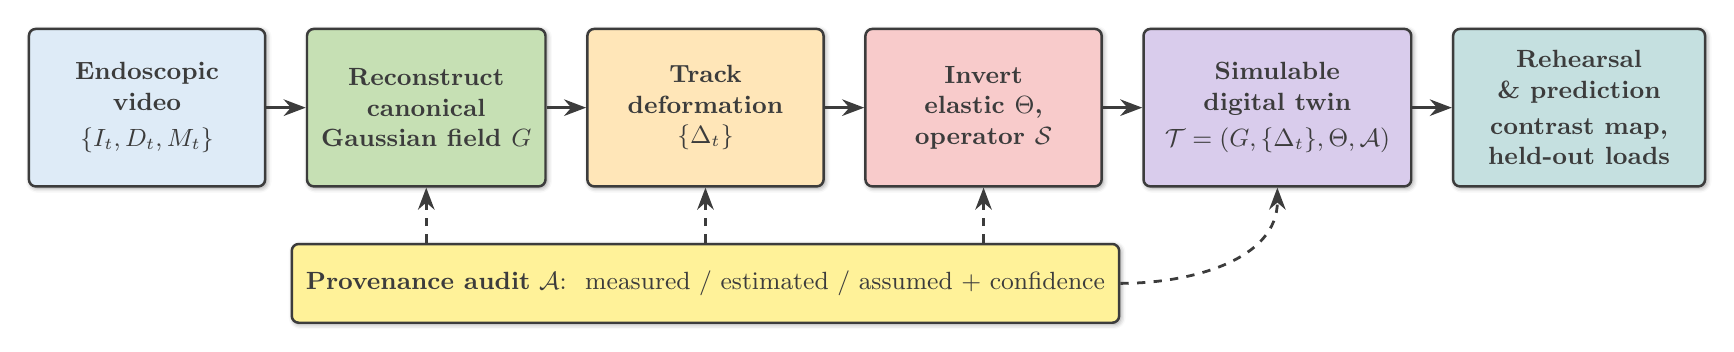
\begin{tikzpicture}[node distance=5mm]

% ===== horizontal main flow =====
\node[stage, fill=cIn] (input)
  {\textbf{Endoscopic}\\ \textbf{video}\\[2pt] $\{I_t,D_t,M_t\}$};

\node[stageT, fill=cT1, right=of input] (t1)
  {\textbf{Reconstruct}\\ canonical\\ Gaussian field $G$};

\node[stageT, fill=cT2, right=of t1] (t2)
  {\textbf{Track}\\ deformation\\ $\{\Delta_t\}$};

\node[stageT, fill=cT3, right=of t2] (t3)
  {\textbf{Invert}\\ elastic $\Theta$,\\ operator $\mathcal{S}$};

\node[stageT, fill=cTwin, right=of t3, minimum width=34mm] (twin)
  {\textbf{Simulable}\\ \textbf{digital twin}\\[2pt] $\mathcal{T}=(G,\{\Delta_t\},\Theta,\mathcal{A})$};

\node[stageT, fill=cUse, right=of twin, minimum width=32mm] (use)
  {\textbf{Rehearsal}\\ \textbf{\& prediction}\\[2pt] contrast map,\\ held-out loads};

% ===== audit bar below (spans the three stages) =====
\node[stage, fill=cAudit, below=7mm of t2, minimum width=96mm, minimum height=10mm] (audit)
  {\textbf{Provenance audit} $\mathcal{A}$:\; measured / estimated / assumed + confidence};

% ===== arrows =====
\draw[arr] (input) -- (t1);
\draw[arr] (t1) -- (t2);
\draw[arr] (t2) -- (t3);
\draw[arr] (t3) -- (twin);
\draw[arr] (twin) -- (use);

% audit dashed connections up to the three stages
\draw[arr, dashed] (audit.north -| t1.south) -- (t1.south);
\draw[arr, dashed] (audit.north -| t2.south) -- (t2.south);
\draw[arr, dashed] (audit.north -| t3.south) -- (t3.south);
\draw[arr, dashed] (audit.east) to[out=0,in=-90] (twin.south);

\end{tikzpicture}
\end{document}
